\documentclass[]{article}
\usepackage{hyperref}
\usepackage[margin=1in]{geometry}
\usepackage{setspace}
\usepackage{float}
\usepackage{graphicx}
\onehalfspacing
%opening
\title{Setting up {\LaTeX} on your computer}
%\author{}

\setlength\parindent{0pt}

\begin{document}

\maketitle
\section*{Installing {\LaTeX} on your computer}
There are many different software you can use to run {\LaTeX} and there is websites where you can run your {\LaTeX} code as well. We will show in this document how to get started with TeXstudio, but feel free to use any other method of your choice if you have one.

To setup {\LaTeX} on your computer, you need \textbf{two} software installed. Depending on your computer system, please follow the instructions below:

\subsection*{Windows Users}
Please make sure you have MikTex 2.9 and TeXStudio installed on your computer. Please install MikTeX first and then install TeXStudio. \\

\textbf{For MikTex 2.9 -}
\begin{enumerate}
\item If disk space is not a problem, please download MikTex Net Installer and do a ``Complete Installation''. This takes about 2GB of computer space. 

\item If disk space is a problem, please download Basic MikTex Installer. This takes about 160ish MB of your disk space. 
\end{enumerate}

\textbf{For TexStudio -  }
Please go to \url{http://www.texstudio.org/} and download TeXStudio 2.12.4(Windows-Installer). 

\subsection*{Mac Users}
Please make sure you have MacTeX and TexStudio installed on your computer. Please install MacTeX first and then install TeXStudio.  \\

\textbf{For MikTex/MacTex:}
Please download and install MacTeX from this link: \url{http://tug.org/mactex/} \\

\textbf{For TexStudio:}
Please download and install TeXStudio from this link: \url{http://www.texstudio.org/} \\

\textit{Please note:} Because TeXStudio does not have an Apple Developer Account, OS X may complain about an unidentified developer and deny opening TeXStudio. In that case, open the context menu on the TeXStudio icon (Ctrl + Click) and select open.

\subsection*{Ubuntu Users}

1) Please go to your Terminal and type the following:
\begin{verbatim}
sudo apt-get install texlive-full
sudo apt-add-repository ppa:blahota/texstudio 
sudo apt-get update 
sudo apt-get install texstudio
\end{verbatim}


\section*{Checking to see if the software are properly installed}

The \texttt{HelloWorld} file is a \texttt{.tex} file that can be used to check if \textbf{TeXstudio} is properly installed on your computer. \\

\textbf{To test it, open the file in TeXstudio and click Build and View in the Tools menu at the top. } \\

If you do not get any error messages (however, you might be asked to install multiple packages the first time you try. Please press install if you get any messages.) and you can see pdf document on the right side of your screen,  then TeXstudio is properly set up for the material in this repository. 

\section*{Adding spellcheck and thesaurus to your TeXStudio}

\subsection*{To install spellcheck dictionary}
To install spell check for English on your TeXStudio, please follow the following steps:

\begin{itemize}
	\item Download the dictionary file from \url{https://extensions.libreoffice.org/extensions/english-dictionaries/2017-05.01/@@download/file/dict-en-20170501.oxt}. Save this file to a folder which you will remember.
	\item On your TeXStudio, go to the \texttt{Options} menu and click on \texttt{Configure TexStudio}.
	\item On the \texttt{Configure TexStudio} settings box that appears, click on \texttt{Language Checking} that appears on the left hand side menu. 
	\item On \texttt{Language Checking}, click on the small blue open button next to the Spelling Dictionaries Directory and point to the folder where you downloaded the file. See Figure 1 for illustrations.
	\item Your dictionary installation is complete!
\end{itemize}

\begin{figure}[H]
	\centering
	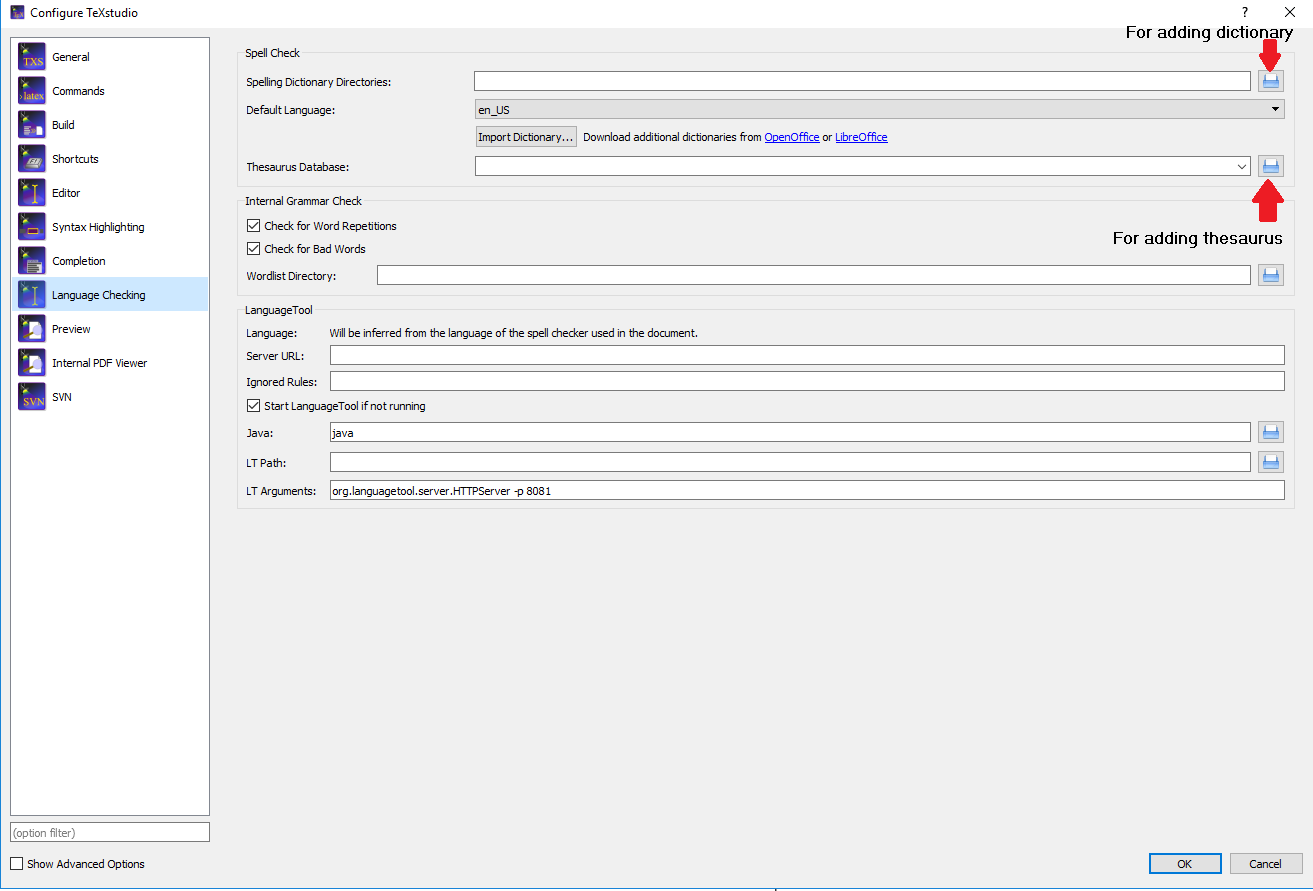
\includegraphics[scale = 0.5]{img/languagetool}
	\caption{Adding dictionaries and thesaurus to TeXStudio}
\end{figure}

\subsection*{To install thesaurus}
 To install thesaurus on your TeXStudio, please follow the following steps:
 \begin{itemize}
 	\item Download the thesaurus file from \url{http://lingucomponent.openoffice.org/MyThes-1.zip}
 	\item Extract the zip file to a folder which you will remember.
 	\item On your TeXStudio, go to the \texttt{Options} menu and click on \texttt{Configure TexStudio}.
 	\item On the \texttt{Configure TexStudio} settings box that appears, click on \texttt{Language Checking} that appears on the left hand side menu. 
 	\item On \texttt{Language Checking}, click on the small blue open buttom  next to the \texttt{Thesaurus Database} and point to the folder where you extracted the downloaded file. See figure 1 for illustrations.
 	\item Your thesaurus installation is complete! 
 \end{itemize}
\end{document}
